%!TEX root = Thesis_main.tex

\chapter{Model of the Mobile Manipulator}
\label{chapter2}
\section{Mobile Robot Model}
\subsection{Holonomic and Nonholonomic constraints}
Considering a system of $N$ rigid bodies and assuming that all of them can reach any position in the space, in order to define uniquely the position of all the bodies of the system, it is necessary to define a vector of $6N = s$ parameters. This set of parameters is termed \textit{generalized coordinates of the unconstrained system}. 
Constraints acting on the position (configuration) of the system are said to be  \textit{holonomic}. 
Holonomic constraints are expressed in the form:
\begin{equation}
h\left( x,q \right) =0
\end{equation}
where $h$ is a vector of dimension $k<s$.
The constraints on the velocities of the system of rigid bodies but not their positions are called \textit{nonholonomic}. In general all constraints which are nonintegrable are said to be nonholonomic, so also inequality constraints about the configuration are considered nonholonomic. 
Nonholonomic constraints reduce the mobility of the mechanical system in a completely different way with respect to holonomic constraints. The fact that the constraint is nonintegrable means that there is no loss of accessibility to the entire configuration space for the system. In other words, while the number of DOFs decreases due to the constraint, the number of generalized coordinates cannot be reduced. Only the subspace of the generalized velocities is reduced.
Nonholonomic constraints are expressed in the form:
\begin{equation}
h( x,\dot{x},q) =0
\end{equation}
where $h$ is a vector of dimension $s<m$.
On the assumption that $h$ has continuous and continuously differentiable components, and its Jacobian $ \partial h/\partial x $ has full rank, the constraints equations allow the elimination of $k$ out of $s$ coordinates of the system. With the remaining $n=s-k$ coordinates it is possible to determine uniquely the configurations of the system satisfying the constraints. Such coordinates are the \textit{generalized coordinates of the constrained system}.\\
Kinematic constraints both holonomic or nonholonomic are usually written in the Pfaffian form, i.e. linearly with respect to the generalized velocities.
\begin{equation}
a_i^T \left( q \right)\dot{q} =0 \qquad i=1,...,k<n 
\end{equation}
\begin{equation*} 
A^T \left( q \right)\dot{q} =0  
\end{equation*}
Assuming now to have $k$ nonholonomic constraint equations for a $n$ dimensional system, this implies that the admissible generalized velocities $\dot{q}$ of the system in any of its configuration $q$ necessarily belong to a $(n-k)$-dimensional space. Specifically, expressing the constraint equations in Pfaffian form, the generalized velocities should belong to the null space of matrix $A^T$.\\
Thus, it can be written:
\begin{equation} \label{G}
\dot{q}=\sum_{j=1}^{m} g_j(q)u_j=G(q)u \qquad m=n-k
\end{equation}
Where $q\in \mathbb{R}^n $ is the state vector, $u= \left[
\begin{matrix}
u_1 &  \cdots & u_m
\end{matrix}
\right]^T\in\mathbb{R}^m $ is the input vector and $\left\lbrace  g_1 (q) \cdots g_m (q) \right\rbrace $ is a basis of the null space of $A^T$, named \textit{input vector fields}. \\
The choice of the input vector fields is not unique, since the input u can have different meanings: velocities, torques or others.\\ 
Talking about mobile robots, wheels are by far the most common mechanism to achieve locomotion. Any wheeled vehicle is subject to kinematic pure rolling constraints that reduce in general its local mobility, while leaving intact the possibility of reaching arbitrary configurations by appropriate manoeuvres. The pure rolling constraint is nonholonomic, because it implies no loss of accessibility in the configuration space of the vehicle.\\
\subsection{Kinematics}
The kinematics of a wheeled mobile robot subjected to pure rolling constraints changes depending on how locomotion is achieved. Mainly there are two types of wheeled mobile robots models: unicycle like robots and bicycle like ones. We'll focus on the first one.
\subsubsection{Unicycle Model}
\begin{figure}[h!]
	\centering
	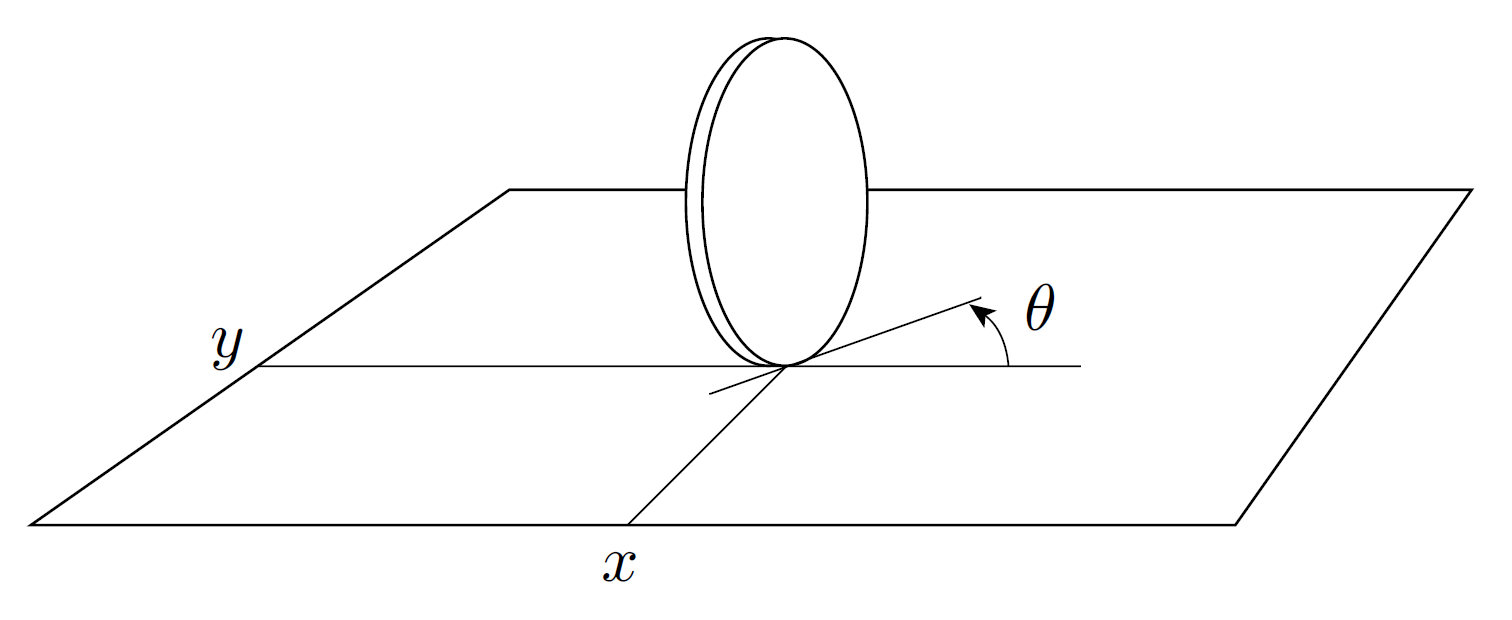
\includegraphics[scale=0.4]{unicycle_model}
	\caption{Unicycle model}
\end{figure}
A unicycle is a vehicle which configuration is completely described by the state vector $q = \left[\begin{matrix}x&y&\theta\end{matrix}\right]^T$, where $x$ and $y$ are the Cartesian coordinates of the contact point of the wheel with the ground and $\theta$ is the orientation of the wheel with respect to the $x$ axis. \\
The constraint of pure rolling for the unicycle is simply expressed as:
\begin{equation} 
\dot{x}\sin\theta-\dot{y}\cos\theta=\left[
\begin{matrix}
\sin\theta & cos\theta & 0
\end{matrix}
\right] \dot{q}=0
\end{equation}
\begin{equation*} \label{At}
A^T \left( q \right)\dot{q} =0  
\end{equation*}
This equation expresses that the velocity of the contact point (or of the wheel centre) is zero in the direction orthogonal to the sagittal axis of the disk.\\
Hence the unicycle is a 3-dimensional subject to one nonholonomic constraint, so the dimension of the basis of the null space of $A^T$ is 2. Choosing:
\begin{equation} \label{Gmatrix_def}
G(q)=\left[
\begin{matrix}
g_1 (q) & g_2 (q)
\end{matrix}
\right] =  \left[
\begin{matrix}
\cos\theta & 0 \\
\sin\theta & 0 \\
0 & 1 
\end{matrix}
\right] 
\end{equation}
All the generalized velocities of the unicycle at $q$ are a combination of $g_1 (q)$ and $g_2 (q)$.
\begin{equation} 
\dot{q}=\left[
\begin{matrix}
\dot{x} \\ \dot{y} \\\dot{\theta}
\end{matrix}
\right] =  \left[
\begin{matrix}
\cos\theta \\ \sin\theta \\ 0 
\end{matrix}
\right]v + \left[
\begin{matrix}
0 \\ 0 \\ 1 
\end{matrix}
\right]\omega
\end{equation}
Where $v$ is the driving velocity, i.e. the velocity of the disk along its sagittal plane, and $\omega$ is the steering velocity, i.e. the angular speed around its vertical axis.\\
A lot of mobile robots are kinematically equivalent to a unicycle, like differential drive robots, skid steering robots or synchro drive vehicles.\\
In most of the unicycle-like mobile robots, $v$ and $\omega$ are the command input to the system, while the actual velocity input are $\omega_R$ and $\omega_L$, i.e. the right and left wheels angular speeds. 
\begin{equation}
v=\frac{r\left(\omega_R + \omega_L\right)}{2} \qquad \omega=\frac{r\left(\omega_R - \omega_L\right)}{d}
\end{equation}
\begin{equation}
\omega_R =\frac{1}{r}\left(v+\frac{d}{2}\omega\right) \qquad \omega_L=\frac{1}{r}\left(v-\frac{d}{2}\omega\right)
\end{equation}
Where $r$ is the wheels radius and $d$ is the distance between their centres.

\subsection{Dynamics}
The dynamic model of a mobile robot can be derived using the Lagrangian formulation for a $n$-dimensional system, defining the Lagrangian $\mathcal{L}$ of the mechanical system as the difference between kinetic and potential energy.
\begin{equation}
\mathcal{L}(q,\dot{q})=\mathcal{T}(q,\dot{q})-\mathcal{U}(q)=\frac{1}{2}\dot{q}^T B(q)\dot{q} - \mathcal{U}(q)
\end{equation}
Where $B(q)$ is the inertia matrix, which is symmetric and positive definite.\\
Writing the Lagrange equations:
\begin{equation}
\frac{d}{dt}\left(\frac{\partial\mathcal{L}}{\partial\dot{q}} \right) - \left(\frac{\partial\mathcal{L}}{\partial q} \right)^T=S(q)\tau+A(q)\lambda
\end{equation}
In this formulation we are adding the energetical term due to the kinematic constraints adding the \textit{Lagrange multipliers} term. 
Substituting the Lagrangian term, we obtain the dynamic model of the mobile base:
\begin{equation}
B(q)\ddot{q}+C(q,\dot{q})\dot{q}+g(q) = S(q)\tau+A(q)\lambda
\end{equation}
\begin{equation*} 
A^T \left( q \right)\dot{q} =0  
\end{equation*}
Where:
\begin{equation}
g(q) = \frac{\partial\mathcal{U}(q)}{\partial q} = 0
\end{equation}
The potential energy of a mobile base during its motion can be considered constant, so it is possible to disregard its derivative.\\
It is possible to further simplify the dynamic model exploiting a useful property of the kinematic relation \ref{G}. Since we defined the coloums of $G(q)$ as vectors belonging to the null space of $A(q)^T$, the following relation holds:
\begin{equation}
G(q)^T A(q) = 0
\end{equation}
So, premultiplying the dynamic model by $G(q)^T$:
\begin{equation} \label{premultiplicationbyG}
G^T(q)\left(B(q)\ddot{q}+C(q,\dot{q})\dot{q}\right) = G^T(q)S(q)\tau
\end{equation}
Reducing the $n$ differential equations to a system of $m$ differential equations without Lagrange multipliers.

\subsubsection{Unicycle Model}
\begin{figure}[h!]
	\centering
	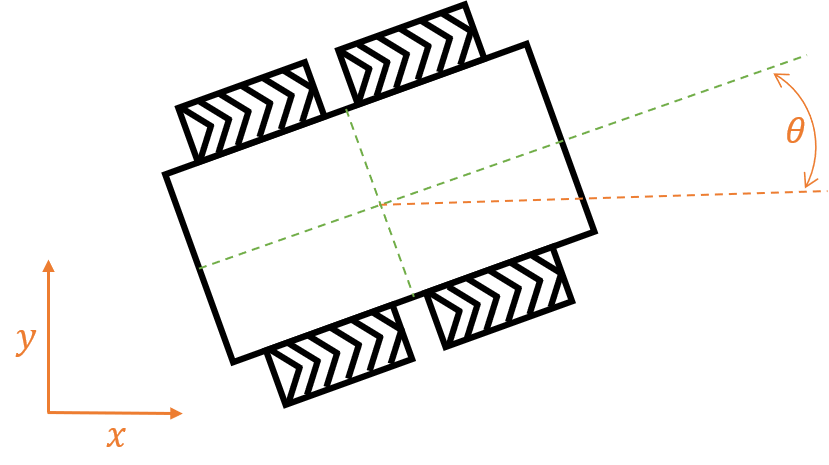
\includegraphics[scale=0.7]{mobile_base}
	\caption{Scheme of a Differential Drive Mobile Robot}
	\label{mobile_base}
\end{figure}
In a unicycle case, like a differential drive robot (Figure \ref{mobile_base}), the dynamic model is very simple if we consider the centre of gravity in the geometric centre of the mobile robot, having:
\begin{equation}
B(q) = \left[\begin{matrix}
M & 0 & 0\\ 0 & M & 0 \\ 0 & 0 & J
\end{matrix} \right]
\qquad 
C(q,\dot{q}) = \left[\begin{matrix}
0 & 0 & 0\\ 0 & 0 & 0 \\ 0 & 0 & 0
\end{matrix} \right]
\end{equation} 
Where $M$ and $J$ are respectively the base’s mass and moment of inertia along its vertical axis $z$.\\
Taking the kinematic equation of the unicycle model, deriving it and substituting it in the dynamic model \ref{premultiplicationbyG} we obtain:
\begin{equation}\label{base_kin_mod}
\dot{q}=G(q)\left[
\begin{matrix}
v_{long} \\ \omega
\end{matrix}
\right] =G(q)v
\end{equation}
\begin{equation}
\ddot{q}=\dot{G}(q)v+G(q)\dot{v}
\quad
\end{equation}
\begin{equation}
\tilde{B}(q)\dot{v}+\tilde{C}(q,\dot{q})v = \tilde{S}(q)\tau
\end{equation}
Where:
\begin{align*}
&\tilde{B}(q) = G^T(q)B(q)G(q) \\
&\tilde{C}(q,\dot{q}) = G^T(q)B(q)\dot{G}(q,\dot{q}) \\
&\tilde{S}(q) = G^T(q)S(q) 
\end{align*}

\section{Manipulator Model}
\subsection{Kinematics}
A manipulator consists of a series of rigid links connected by joints. In order to plan the manipulator motion from an initial to a final configuration, i.e. the set of joint values, it is necessary to define its pose with respect to a reference frame. 
\subsubsection{Rototraslation Matrices}
Considering two different reference frames: $x^0,y^0,z^0$ and $x^1,y^1,z^1$ with two different origins $O^0$ and $O^1$, a point P is represented by the two frames respectively with vectors $p^0$ and $p^1$.
\begin{figure}[h!]
	\centering
	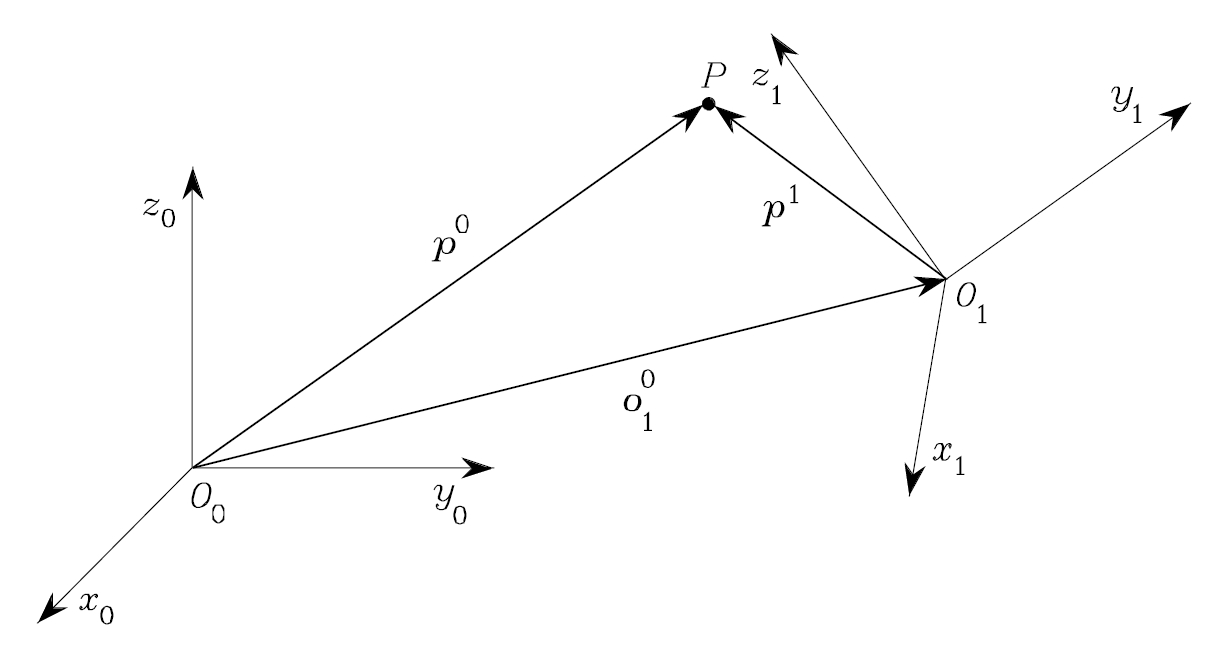
\includegraphics[scale=0.5]{rototraslation_frames}
	\caption{}
\end{figure}
The vector $p^0$ can be represented as the sum of two vectors:
\begin{equation} \label{rototrasl}
	p^0= o_1^0 + R_1^0 p^1
\end{equation}
Where $R^0_1$ is the rotation matrix of frame $x^1,y^1,z^1$ with respect to frame $x^0,y^0,z^0$ and so $R_1^0 p^1$ is the representation of vector $p^1$ in the frame $x^0,y^0,z^0$.\\
It is possible to express the equation above in a compact form using the homogenous transformation matrix simply defining:
\begin{equation} \label{A}
	\tilde{p}=\left[
	\begin{matrix}
	p\\ 1
	\end{matrix}
	\right] \qquad 
	A_1^0 = \left[
	\begin{matrix}
       R_1^0 & o_1^0 \\ [0] & 1
	\end{matrix}
	\right]
\end{equation}
\begin{equation}
	\tilde{p}^0 = A_1^0\tilde{p}^1
\end{equation}
The matrix $A_1^0$ is called \textit{rototraslation matrix}.\\
Inverting the equation \ref{rototrasl} we can express the inverse transformation.
\begin{equation} 
p^1= -R_0^1o_1^0 + R_0^1 p^0
\end{equation}
\begin{equation}
	A_0^1 = \left[
	\begin{matrix}
		R_0^1 & -R_0^1o_1^0 \\ [0] & 1
	\end{matrix}
	\right]
\end{equation}
Where:
\begin{equation*}	
	R_0^1 = (R_1^0)^{-1}=(R_1^0)^{T}
\end{equation*}
\begin{equation*}
A_0^1 = (A_1^0)^{-1}
\end{equation*}
Both with rotation and rototraslation matrices, it is possible to obtain a composition of consecutive transformations by postmultiplying the matrices related to the single rotations:
\begin{align}
	R_2^0 = R_1^0R_2^1\\
	A_2^0 = A_1^0A_2^1	
\end{align}

\subsubsection{Denavit-Hartenberg Parameters}
Since the first ‘80s a popular approach to describe the kinematics of robots, and therefore the rototraslation matrices to express the transformation from one joint frame to the following, is the convention introduced by Jacques Denavit and Richard Hartenberg in 1955 for a compact description of mechanisms.  
Their representation is based on the concept of the common normal between joint axes, defined as the shortest line between two axes, perpendicular to both axes. 

\begin{figure}[h!]
	\centering
	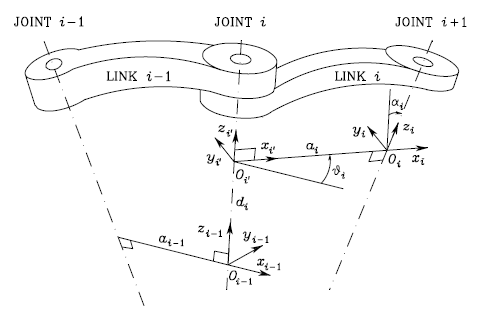
\includegraphics[scale=0.5]{denavit_hartenberg}
	\caption{Denavit-Hartenberg convention for Robot links}
\end{figure}

The convention firstly assigns to each link a reference frame referring to the following rules: 
\begin{itemize}
	\item Axis $z_i$ is chosen along the axis of joint i+1;
	\item The origin $O_i$ is located at the intersection of axis $z_i$ with the common normal to axes $z_{i-1}$ and $z_i$;
	\item Axis $x_i$ is chosen as an extension of the common normal to axes $z_{i-1}$ and $z_i$;
	\item Axis $y_i$ is chosen to complete a right-handed frame.
\end{itemize}
Once established a frame for each link, 4 parameters describe the pose of frame i with respect to frame i-1.
\begin{itemize}
	\item $a_i$ : distance between $z_i$ and $z_{i-1}$. Only geometrical, depends only on the geometry of the links
	\item $d_i$ : coordinate of $O_i$ along $z_{i-1}$. Varies if the joint is prismatic.
	\item $\alpha_i$: angle between axes $z_{i-1}$ and $z_i$ (positive counterclockwise with respect to axis $x_i$). Only geometrical, depends only on the geometry of the links.
	\item $\theta_i$: angle between axes $x_{i-1}$ and $x_i$ (positive counterclockwise with respect to axis $z_{i-1}$). Varies if the joint is revolute.
\end{itemize}
The transformation matrix between frame i and frame i-1 can then be built:
\begin{equation}
	A_i^{i-1}(q_i)=\left[
	\begin{matrix}
		\cos\theta & -\sin\theta\cos\alpha & \sin\theta\sin\alpha & a\cos\theta \\
		\sin\theta & \cos\theta\cos\alpha & -\cos\theta\sin\alpha & a\sin\theta \\
		0 & \sin\alpha & \cos\alpha & d \\
		0 & 0 & 0 & 1
	\end{matrix}
	\right]
\end{equation}
This matrix is function only of the joint variables $\theta$ and $d$.

\subsubsection{Direct and Inverse Kinematics} \label{dirinvkin}
As anticipated, a manipulator is basically made of links chained together by joints that connect the \textit{base} of the manipulator to its \textit{end effector}.\\
The \textit{direct kinematics} of the manipulator express the position and orientation of the end effector as a function of the robot configuration. Using the concepts showed up to this point, this corresponds to the definition of the rototraslation matrix that describes the end effector frame with respect to the global reference frame:
\begin{equation}\label{AAAA}
	A_{ee}^{base}=A_1^{base}A_2^1A_3^2\cdots A_{ee}^{ee-1}
\end{equation}
The opposite problem is the definition of the \textit{inverse kinematics}, i.e. given the position and orientation of the end effector, finding the corresponding joint variables. The inverse kinematics problem is not easy to solve since it is often nonlinear and there can be infinite solutions as well as none.\\
An important concept which roboticists are still working on is \textit{kinematic redundancy}, i.e. when the number of joint variables is greater than the dimension of the operational space relative to the task to be achieved. For example for a problem of end effector position and orientation regulation the task opertaional space is 6-dimensional.
When a system is kinematically redundant, direct kinematics is always possible to be defined, while inverse kinematics can have infinite solutions.
Solving the \textit{kinematic redundancy problem} means to define a criterion in order to be able to pick one among the infinite configurations which have the end effector in the same position and orientation.\\
This concept will be very important in the defintion of Mobile Manipulator control.
\subsection{Dynamics}
\label{sec:dynamics}
As we already seen in the case of mobile robots the dynamics of a robot can be expressed with the Euler-Lagrange formulation.
\begin{equation*}
	\mathcal{L}=\mathcal{T}-\mathcal{U}
\end{equation*}
\begin{equation*}
	\frac{d}{dt}\left(\frac{\partial\mathcal{L}}{\partial\dot{q}} \right) - \left(\frac{\partial\mathcal{L}}{\partial q} \right)^T=\tau
\end{equation*}
Where $q$ is the vector of the generalized coordinates and $\tau$ is the vector of the generalized forces.\\
The potential energy of the manipulator is given by
\begin{equation}
	\mathcal{U} = \sum_{i=1}^{n}\left(\mathcal{U}_{l_i}+\mathcal{U}_{m_i}\right)
\end{equation}
Where $\mathcal{U}_{l_i}$ and $\mathcal{U}_{m_i}$ are the potential energy due to the gravitational forces of the links and of the motors respectively.\\
Similarly, the kinetic energy of the entire system is the sum of the kinetic energies of the links and of the motors 
\begin{equation}
	\mathcal{T} = \sum_{i=1}^{n}\left(\mathcal{T}_{l_i}+\mathcal{T}_{m_i}\right)
\end{equation}
In order to relate the velocities of every elementary particle of the manipulator to the joint velocities we have to express in a proper way the Jacobians.
\begin{align}
	{\dot{\mathbf{p}}}_{l_i}=\mathit{j}_{P_1}^{(l_i)}{\dot{q}}_1+\mathit{j}_{P_2}^{(l_i)}{\dot{q}}_2+\cdots+\mathit{j}_{P_i}^{\left(l_i\right)}{\dot{q}}_i=\mathcal{J}_P^{(l_i)}\dot{q}
	\\
	\omega_{l_i}=\mathit{j}_{O_1}^{(l_i)}{\dot{q}}_1+\mathit{j}_{O_2}^{(l_i)}{\dot{q}}_2\cdots+\mathit{j}_{O_i}^{\left(l_i\right)}{\dot{q}}_i=\mathcal{J}_O^{(l_i)}\dot{q}
\end{align}

Where with $\mathcal{J}_P^{(l_i)}$ we mean the Jacobian matrix relating the generalized joint velocities to the linear velocity of the centre of mass of link $i$, and with $\mathcal{J}_O^{(l_i)}$ we mean the Jacobian matrix relating the generalized joint velocities to the angular velocity of the centre of mass of link $i$. 
The columns of the Jacobian matrices are:
\begin{equation}
	\mathit{j}_{P_j}^{(l_i)}=
	\begin{cases}
		z_{j-1} & \text{for a \textit{prismatic} joint} \\
		z_{j-1}\times \left(\mathbf{p}_{l_i}-\mathbf{p}_{j-1}\right) & \text{for a \textit{revolute} joint}	
	\end{cases}                                             
\end{equation}
\begin{equation}
	\mathit{j}_{O_j}^{(l_i)}= 
	\begin{cases}
		0 & \text{for a \textit{prismatic} joint} \\
		z_{j-1} & \text{for a \textit{revolute} joint}	
	\end{cases} 
\end{equation}
So it is possible to express the kinetic energy as:
\begin{equation}\label{iniziodinamica}
	\mathcal{T}= \frac{1}{2}\sum_{i=1}^{n}\sum_{j=1}^{n}{b_{ij}(q){\dot{q}}_i{\dot{q}}_j}=\frac{1}{2}{\dot{q}}^TB\left(q\right)\dot{q}
\end{equation}
Where:
\begin{align*}
	B\left(q\right)=\sum_{i=1}^{n} &m_{l_i}{\mathcal{J}_P^{(l_i)}}^T\mathcal{J}_P^{(l_i)}+\frac{1}{2}{\mathcal{J}_O^{(l_i)}}^TR_iI_{l_i}^iR_i^T\mathcal{J}_O^{(l_i)} \\
	+&m_{m_i}{\mathcal{J}_P^{(m_i)}}^T\mathcal{J}_P^{(m_i)}+{\mathcal{J}_O^{(m_i)}}^TR_{m_i}I_{m_i}^{m_i}R_{m_i}^T\mathcal{J}_O^{(m_i)} 
\end{align*}
Is the $(n\times n)$ symmetric positive-definite inertia matrix of the system, with $m_{l_i}$ and $m_{m_i}$ as the mass of link and motor $i$ and $I_{l_i}^i$ and $I_{m_i}^{m_i}$ as the inertia tensor of the the link and motor $i$ with respect to the $i$th reference frame.\\
Recovering the Lagrange equation:
\begin{equation*}
	\frac{d}{dt}\left(\frac{\partial \mathcal{L}}{\partial\dot{q}}\right)^T-\left(\frac{\partial \mathcal{L}}{\partial q}\right)^T=\tau
\end{equation*}
\begin{equation}
	\begin{split}
		\frac{d}{dt}\left(\frac{\partial \mathcal{T}}{\partial\dot{q_i}}\right)-\left(\frac{\partial \mathcal{T}}{\partial q_i}\right)=
		\sum_{j=1}^{n}{b_{ij}\left(q\right){\ddot{q}}_j}+\sum_{j=1}^{n}\sum_{k=1}^{n}{\frac{{\partial b}_{ij}\left(q\right)}{\partial q_k}{\dot{q}}_k{\dot{q}}_j}&\\-\frac{1}{2}\sum_{j=1}^{n}\sum_{k=1}^{n}{\frac{\partial b_{jk}(q)}{\partial q_i}{\dot{q}}_k{\dot{q}}_j}&\\
		=\sum_{j=1}^{n}{b_{ij}\left(q\right){\ddot{q}}_j}+\sum_{j=1}^{n}\sum_{k=1}^{n}{h_{ijk}\left(q\right){\dot{q}}_k{\dot{q}}_j}&
	\end{split}
\end{equation}
\begin{equation}
	\frac{d}{dt}\left(\frac{\partial \mathcal{T}}{\partial\dot{q}}\right)^T-\left(\frac{\partial \mathcal{T}}{\partial q}\right)^T=B(q)\ddot{q}+C\left(q,\dot{q}\right)\dot{q}
\end{equation}
Where $C\left(q,\dot{q}\right)$ is the non-symmetric positive definite Coriolis matrix that represents the effect of motion of joint $j$ and $k$ on the motion of joint $i$. 
\\Considering the potential energy within the Lagrange equation.
\begin{equation*}
	\mathcal{U}=\sum_{i=1}^{n}{(\mathcal{U}_{l_i}+\mathcal{U}_{m_i})}
\end{equation*}
\begin{equation}
	\mathcal{U}_{l_i}=-m_{l_i}\mathbf{g}_0^T\mathbf{p}_{l_i}\ \ \ \ ,\ \ \ \ \mathcal{U}_{m_i}=-m_{m_i}\mathbf{g}_0^T\mathbf{p}_{m_i}
\end{equation}

Where $\mathbf{g}_0$ is the gravity acceleration vector. So:
\begin{equation}
	\frac{\partial \mathcal{U}}{\partial q_i}=-\sum_{j=1}^{n}\left(m_{l_i}\mathbf{g}_0^T\frac{{\partial\mathbf{p}}_{l_i}}{\partial q_i}+m_{m_i}\mathbf{g}_0^T\frac{{\partial\mathbf{p}}_{m_i}}{\partial q_i}\right)=g_i(q)
\end{equation}
So the final equation of the manipulator dynamic model is:
\begin{equation}\label{dynamics}
	B\left(q\right)\ddot{q}+C\left(q,\dot{q}\right)\dot{q}+g\left(q\right)=\ \tau
\end{equation}
Where $g(q)$ is the gravitational vector that represents the moments acting on the joints due to gravity force.

\section{Mobile Manipulator Model}
\subsection{Kinematics}
\begin{figure}
\centering
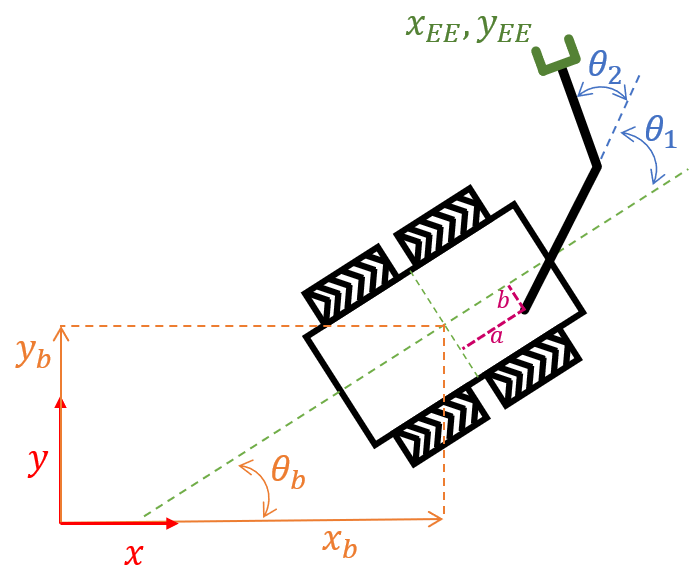
\includegraphics[scale=0.8]{MM_kinematics}
\label{MM_kin}
\caption{A simple Mobile Manipulator composed by a mobile base and a 2-DoF robotic arm}
\end{figure}
Considering the general case of a mobile manipulator composed by a manipulator arm mounted on a mobile platform, its kinematic model set the location of the end effector as a function of both the arm and base generalized coordinates.
\begin{equation}\label{dirkinMM}
	X_{EE}=\left[\begin{matrix}\mathbf{p}_{EE}\\\Phi\end{matrix}\right]=f(q)=f\left(\left[\begin{matrix}q_b\\q_a \end{matrix}\right]\right)
\end{equation}
Where $\mathbf{p}_{EE}=\left[\begin{matrix}x_{EE}&y_{EE}&z_{EE}\end{matrix}\right]^T$ is the vector of the end effector position and $\Phi =\left[\begin{matrix}\vartheta_{EE}&\varphi_{EE}&\psi_{EE}\end{matrix}\right]$ is the vector of the end effector orientation that can be expressed with different conventions like Azimut-Elevation-Rotation, or Roll-Pitch-Yaw. As an example, the forward kinematics for just the Cartesian coordinates of the end effector of the simplified system in figure \ref{MM_kin} is
\begin{equation*}
\begin{split}
	x_{EE}&=x_b+a\cos\theta-b\sin\theta+l_1\cos\left(\theta+\theta_1\right)+l_2\cos\left(\theta+\theta_1+\theta_2\right)\\
	y_{EE}&=y_b+a\sin\theta-b\cos\theta+l_1\sin\left(\theta+\theta_1\right)+l_2\sin\left(\theta+\theta_1+\theta_2\right)
\end{split}
\end{equation*}
It is possible to define the function $f(q)$ of Eq.\ref{dirkinMM} premultiplying the rototranslation matrix $A_{base}^{global}$, relative to the mobile base motion, to the direct kinematics of the arm. In the case of the previous example:
\begin{equation}
	A_{base}^{global}=\left[\begin{matrix}
		\cos\theta&-\sin\theta&0&x_b+a\cos\theta-b\sin\theta\\
		\sin\theta&\cos\theta&0&y_b+a\sin\theta-b\cos\theta\\
		0&0&1&h_{base}\\
		0&0&0&1
	\end{matrix}\right]
\end{equation}
So the forward kinematics can be obtained consequently:
\begin{equation}
A_{ee}^{global}=A_{base}^{global}A_1^{base}A_2^1\cdots A_{ee}^{ee-1}
\end{equation}
\subsubsection{Redundancy}
As we had briefly introduced before, a robot is kinematically redundant if the number of its degrees of freedom is greater than it is strictly necessary. In this sense redundancy is thus a concept relative to the given task. Mobile Manipulators are systems specifically built redundant in order to exploit the extra degrees of freedom to:
\begin{itemize}
	\item avoid collision with obstacles;
	\item avoid kinematic singularities;
	\item increase the manipulability of the system;
	\item move with lower joint velocities;
	\item etc.
\end{itemize}
Anyway redundancy is an issue when dealing with inverse kinematics since infinite solutions exist. So, solutions are mainly sought at velocity levels.
\subsubsection{Differential kinematics}
Differentiating $f$, the differential forward kinematics of the Mobile Manipulator can be obtained. 
\begin{equation}\label{eq:dotx_EE}
	\dot{X}_{EE}=\mathcal{J}_b(q)\dot{q}_b+\mathcal{J}_a(q)\dot{q}_a
\end{equation}
Where the columns of $\mathcal{J}_a(q)=\frac{\partial f}{\partial q_a}(q_a,\theta)$ can be obtained similarly to the way described in section \ref{sec:dynamics}.
\begin{equation}
\mathit{j}_{P_j}^{(EE)}=
	\begin{cases}
	z_{j-1} & \text{for a \textit{prismatic} joint} \\
	z_{j-1}\times \left(\mathbf{p}_{EE}-\mathbf{p}_{j-1}\right) & \text{for a \textit{revolute} joint}	
	\end{cases}                                             
\end{equation}
\begin{equation}
	\mathit{j}_{O_j}^{(EE)}= 
	\begin{cases}
	0 & \text{for a \textit{prismatic} joint} \\
	z_{j-1} & \text{for a \textit{revolute} joint}	
	\end{cases} 
\end{equation}
and $\mathcal{J}_b(q)=\frac{\partial f}{\partial q_b}(q_a,\theta)$ can be obtained at the same way considering $x$ and $y$ as prismatic joints and $\theta$ as a revolute joint of the compound system.\\
In doing this the nonholonomic constraint of the mobile platform \ref{G} should be taken into account:
\begin{equation}
	\mathcal{J}_b(q)\dot{q}_b=\mathcal{J}_b(q)G(q)v=\mathcal{J}_v(\theta)v
\end{equation}
Therefore is now possible to reformulate eq \ref{eq:dotx_EE} in a compact form to express the end effector traslational and rotational velocities as a function of the 8-elements input vector of joints and vehicle velocities.
\begin{equation}
\dot{X}_{EE}=\left[\begin{matrix}
\mathcal{J}_v(\theta) & \mathcal{J}_a(q)
\end{matrix}\right]\left[\begin{matrix}v\\\dot{q_a} \end{matrix}\right]
\end{equation}
\subsection{Dynamics}
Once obtained the expessions of Jacobians $\mathcal{J}^{(l_i)}_b(q)$ and $\mathcal{J}^{(l_i)}_a(q)$, equations from \ref{iniziodinamica} to \ref{dynamics} can be applied to the Mobile Manipulator case as if it were a compound manipulator, obtaining:
\begin{equation}
B\left(q\right)\left[
\begin{matrix}\ddot{q}_b\\\ddot{q}_a\\
\end{matrix}
\right]+C\left(q,\dot{q}\right)\left[
\begin{matrix}
\dot{q}_b\\\dot{q}_a\\
\end{matrix}\right]+g\left(q\right)= \left[
\begin{matrix}
\tau_b\\\tau_a\\
\end{matrix}\right]+\left[
\begin{matrix}
A(q_b)\\0\\
\end{matrix}\right]\lambda
\end{equation}
\begin{equation}
\begin{split}
\left[
\begin{matrix}
B_b(q)&B_{ba}(q)\\
B_{ab}(q)&B_a(q)
\end{matrix}\right]\left[
\begin{matrix}
\ddot{q}_b\\\ddot{q}_a
\end{matrix}\right]&\\ +\left[
\begin{matrix}
C_b(q,\dot{q})&C_{ba}(q,\dot{q})\\
C_{ab}(q,\dot{q})&C_a(q,\dot{q})
\end{matrix}\right]\left[
\begin{matrix}
\dot{q}_b\\\dot{q}_a
\end{matrix}\right] &\\ +\left[
\begin{matrix}
0\\g(q_a)
\end{matrix}\right]	&= \left[
\begin{matrix}
\tau_b\\\tau_a
\end{matrix}\right]+\left[
\begin{matrix}
A(q_b)\\0\\
\end{matrix}\right]\lambda
\end{split}	
\end{equation}
Where also the Lagrange multipliers term has been added to take into account the nonholonomic constraint on the motion of the base. \\Similarly to the transformation done in \ref{premultiplicationbyG}, the following expression can be obtained:
\begin{equation}
\begin{split}
\left[\begin{matrix}G^T(q_b)B_b(q)&G^T(q_b)B_{ba}(q)\\B_{ab}(q)&B_a(q)\\\end{matrix}\right]\left[\begin{matrix}\ddot{x
q}_b\\\ddot{q}_a\\\end{matrix}\right] &\\
+\left[\begin{matrix}G^T(q_b)C_a(q,\dot{q})&G^T(q_b)C_{ba}(q,\dot{q})\\C_{ab}(q,\dot{q})&C_a(q,\dot{q})\\\end{matrix}\right]\left[\begin{matrix}\dot{q}_b\\\dot{q}_a\\\end{matrix}\right] &\\
+\left[\begin{matrix}0\\g(q_a)\\\end{matrix}\right]
&= \left[\begin{matrix}G^T(q_b)\tau_b\\\tau_a\\\end{matrix}\right]
\end{split}
\end{equation}
The columns of $G$ are a basis of the null space of $A(q_b)T$, so the Lagrange multipliers term is set to zero.
If we now consider the kinematic equation of the base \ref{G}:
\begin{equation}
\left[\begin{matrix}\dot{q}_b\\\dot{q}_a\\\end{matrix}\right]=\left[\begin{matrix}G(q_b)&0\\0&I\\\end{matrix}\right]\left[\begin{matrix}v\\\dot{q}_a\\\end{matrix}\right]
\end{equation}
Whose derivative is:
\begin{equation}
\ddot{q}_b=G\left(q_b\right)\dot{v}+\dot{G}\left(\dot{q}_b,q_b\right)v
\end{equation}
\begin{equation}
\left[\begin{matrix}\ddot{q}_b\\\ddot{q}_a\\\end{matrix}\right]=\left[\begin{matrix}G(q_b)&0\\0&I\\\end{matrix}\right]\left[\begin{matrix}\dot{v}\\\ddot{q}_a\\\end{matrix}\right]+\left[\begin{matrix}\dot{G}\left(\dot{q}_b,q_b\right)&0\\0&0\\\end{matrix}\right]\left[\begin{matrix}v\\\dot{q}_a\\\end{matrix}\right]
\end{equation}
If we substitute these expressions in the dynamic model of the mobile manipulator:
\begin{equation} \label{dynamicsMM}
\left[\begin{matrix}G^TB_bG&G^TB_{ba}\\B_{ab}G&B_a\\\end{matrix}\right]\left[\begin{matrix}\dot{v}\\\ddot{q}_a\\\end{matrix}\right]+\left[\begin{matrix}G^TB_b\dot{G}+G^TC_bG&G^TC_{ba}\\B_{ab}\dot{G}+C_{ab}G&C_a\\\end{matrix}\right]\left[\begin{matrix}v\\\dot{q}_a\\\end{matrix}\right]+\left[\begin{matrix}0\\g\\\end{matrix}\right]=\ \left[\begin{matrix}G^T\tau_b\\\tau_a\\\end{matrix}\right]
\end{equation}
Where the parenthesis have not been transcribed in order to have a compact expression.

\subsection{Mixed Kinematics and Dynamics Model}
The idea of the following model is to describe kinematically the mobile base and dynamically the manipulator, in order to have as inputs:
\begin{itemize}\itemsep1pt
	\item[--] the torques applied at the manipulator joints
	\item[--] the longitudinal and angular velocity of the mobile base.
\end{itemize}
$v$, which is the velocity vector of the base, is the input vector of the kinematic model of the base. The idea is to use $v$ and $\dot{v}$ as inputs also in the dynamic model of the manipulator. 
For this purpose, we exploit the fact that the kinematic relations of the mobile base are already been used within the dynamic model of the whole mobile manipulator. \\Focusing on the dynamic equation of only the manipulator part, i.e. the second row of \ref{dynamicsMM}.
\begin{equation}
	\left[\begin{matrix}B_{ab}G&B_a\\\end{matrix}\right]\left[\begin{matrix}\dot{v}\\\ddot{q}_a\\\end{matrix}\right]+\left[\begin{matrix}B_{ab}\dot{G}+C_{ab}G&\quad C_a\\\end{matrix}\right]\left[\begin{matrix}v\\\dot{q}_a\\\end{matrix}\right]+g=\ \tau_a
\end{equation}
Rearranging the terms we obtain:
\begin{equation}
	\left[B_a\right]\ddot{q}_a+\left[C_a\right]\dot{q}_A+g=\tau_a-\left[B_{ab}G\right]\dot{v}-\left[B_{ab}\dot{G}+C_{ab}G\right]v
\end{equation}
Which in state space form is:
\begin{equation}
\begin{split}
	\left[\begin{matrix}\ddot{q}_A\\\dot{q}_a\\\end{matrix}\right]&=\left[\begin{matrix}-{B_a}^{-1}C_a&0\\I&0\\\end{matrix}\right]\left[\begin{matrix}\dot{q}_a\\q_a\\\end{matrix}\right]+\left[\begin{matrix}{{-B}_a}^{-1}g\\0\\\end{matrix}\right]+\left[\begin{matrix}{B_a}^{-1}\\0\\\end{matrix}\right]\tau_a\\&+\left[\begin{matrix}-{B_a}^{-1}B_{ab}G\\0\\\end{matrix}\right]\dot{v}\\&+\left[\begin{matrix}-{B_a}^{-1}\left[B_{ab}\dot{G}+C_{ab}G\right]\\0\\\end{matrix}\right]v
\end{split}
\end{equation}
Adding also the kinematic equation of the base we have the entire model of the system in state space form:
\begin{equation}
	\begin{split}
		\left[\begin{matrix}\ddot{q}_a\\\dot{q}_A\\\dot{q}_b\\\end{matrix}\right]&=\left[\begin{matrix}-{B_a}^{-1}C_a&0&0\\I&0&0\\0&0&0\\\end{matrix}\right]\left[\begin{matrix}\dot{q}_a\\q_a\\q_b\\\end{matrix}\right]+\left[\begin{matrix}{{-B}_a}^{-1}g\\0\\0\\\end{matrix}\right]+\left[\begin{matrix}{B_a}^{-1}\\0\\0\\\end{matrix}\right]\tau_a\\&+\left[\begin{matrix}-{B_a}^{-1}B_{ab}G\\0\\0\\\end{matrix}\right]\dot{v}\\&+\left[\begin{matrix}-{B_a}^{-1}\left[B_{ab}\dot{G}+C_{ab}G\right]\\0\\G\\\end{matrix}\right]v 
	\end{split}
\end{equation}
